\documentclass[11pt]{article}
\usepackage[]{authblk}
\usepackage{graphicx}
\usepackage{color}
\usepackage{longtable}
\usepackage{hanging}
\usepackage{indentfirst}
\usepackage{setspace}
\usepackage{verbatim}
\usepackage{upgreek}
\usepackage{framed}
\usepackage{ textcomp }
\usepackage[weather]{ifsym}
\usepackage{natbib}
\usepackage{url}
\usepackage{soul}
\usepackage{amsmath, amsfonts,amssymb,mathrsfs}
\usepackage{fancyhdr}
\usepackage[compact]{titlesec}
\usepackage[T1]{fontenc}
\usepackage{lmodern}

\setlength{\evensidemargin}{0in}
\setlength{\headheight}{0in}
\setlength{\headsep}{0in}
\setlength{\oddsidemargin}{-0.25in}
\setlength{\paperheight}{11in}
\setlength{\paperwidth}{8.5in}
\setlength{\tabcolsep}{0in}
\setlength{\textheight}{9in}
\setlength{\textwidth}{7in}
\setlength{\topmargin}{0in}
\setlength{\topskip}{0in}
\setlength{\voffset}{0in}
%\setstretch{2}
%\raggedright
\parskip = 0.15in
\pagestyle{plain}
\setlength{\parindent}{0cm}

\definecolor{citescol}{RGB}{194,101,1}
%\definecolor{citescol}{RGB}{73,0,165}
\definecolor{urlscol}{RGB}{0,150,206}
%\definecolor{urlscol}{RGB}{0,107,124}
%\definecolor{linkscol}{RGB}{187,24,0}
\definecolor{linkscol}{RGB}{149,0,207}
%\definecolor{linkscol}{RGB}{73,0,165}
\definecolor{mycol}{RGB}{25,23,191}
\definecolor{outputcol}{RGB}{34,139,34}


%\def\Fld@bordercolor{1 0 0}
%\renewcommand*{\DefaultHeightofTextMultiline}{6\baselineskip} 
%\renewcommand*{\LayoutTextField}[2]{\makebox[6em][l]{#1 }%
%  \raisebox{\baselineskip}{\raisebox{-\height}{#2}}}
%\def\LayoutChoiceField#1#2{\makebox[6em][l]{#1 }#2}

%\LayoutTextField{label}{field}

\DeclareMathAlphabet{\msfsl}{T1}{cmr}{m}{it}
\DeclareMathAlphabet{\msyf}{OMX}{pcr}{m}{it}
\newcommand{\alf}{\upalpha}
\newcommand{\hilight}[1]{\colorbox{yellow}{#1}}

\newcommand{\levelone}[1]{
\bigskip
\noindent{\LARGE{\textsc{#1}}}
\vspace {0.05in}
}

\newcommand{\leveltwo}[1]{
\bigskip
\noindent{\Large{\textit{#1}}}
\vspace {-1mm}
}

\newcommand{\descriptionhead}[1]{
\noindent{\textbf{\textit{#1}}}\\ \vspace{-7mm}
}

\newcommand{\dhead}[1]{
\noindent{\textbf{\textit{#1 --}}}
}


\newcommand{\exs}[1]{
\vspace{-4mm}
\begin{itemize}
\item #1 \\ \vspace{-8mm}
\end{itemize}
}

\newcommand{\nbo}[1]{{\color{red}{#1}}}


\newcommand{\stepbullet}{\noindent \textbullet \ }
\newcommand{\mi}[1]{\textbf{\textit{#1}}}


\newcommand{\levelthree}[1]{\textit{#1 --}}

%\newcommand{\bowtiecirclefig}{{\rlap{\rlap{{\textbf{\BigCircle}}}{\FilledTriangleLeft}}\FilledTriangleRight}}

\bibliographystyle{bib_tex/mbe}
\bibpunct[; ]{(}{)}{;}{a}{,}{;}


\usepackage[breaklinks]{hyperref}
\usepackage[all]{hypcap}
\hypersetup{colorlinks=true,linkcolor=linkscol,citecolor=citescol,urlcolor=urlscol}


\usepackage{framed}
\usepackage{listings}

\lstset{breaklines=true}

\definecolor{shadecolor}{RGB}{238,224,229}


\setlength{\topmargin}{-0.4in}
\setlength{\headheight}{14.5pt}
\pagestyle{fancy}

\newcommand{\taha}[1]{{\textcolor{red}{[TAH comment: #1]}}} % TAH comment

\titlespacing{\section}{0pt}{*0}{*0}
\titlespacing{\subsection}{0pt}{*0}{*0}
\titlespacing{\subsubsection}{0pt}{*0}{*0}

\titleformat{\section}
  {\normalfont\Large\bfseries\color{mycol}}
  {\thesection}{1em}{}

\titleformat{\subsection}
  {\normalfont\large\bfseries\color{mycol}}
  {\thesubsection}{1em}{}

\titleformat{\subsubsection}
  {\normalfont\bfseries\color{mycol}}
  {\thesubsection}{1em}{}

% command for MrBayes command-line step
\newcommand{\cl}[1]{{\texttt{\textbf{#1}}}}

\newcommand{\mbcl}[1]{\exs{\cl{MrBayes > {#1}}}}

\newcommand{\rbprmt}{RevBayes > } 
\newcommand{\rbcl}[1]{\exs{\cl{\rbprmt{#1}}}}
\newcommand{\rbout}[1]{\exs{\cl{\textcolor{outputcol}{#1}}}}
\newcommand{\rbdn}{{\Large \symbol{126}}} % This makes a copy/pasteable tilde
\newcommand{\rbclml}[1]{\exs{\cl{\ \ \ \ \ \ \ \ \ \ \ {#1}}}}




\begin{document}
\renewcommand{\headrulewidth}{0.5pt}
\headsep = 20pt
\lhead{ }
\rhead{\textsc {RevBayes Tutorial --- Model Selection \& Partitioning}}

\thispagestyle{plain}
\begin{center}

\textbf{\LARGE Phylogenetic Inference using RevBayes}\\\vspace{2mm}
\textbf{\it{\Large Model Selection \& Data Partitioning}}\\\vspace{2mm}
\end{center}

\section*{Overview}

RevBayes is a software program for inferring phylogenetic parameters in a Bayesian statistical framework. 
 
\taha{write an overview of RevBayes}

This tutorial demonstrates how to set up and perform an analysis that calculates Bayes factors to select among partitioning schemes...
\taha{add breif description of exercise}


\bigskip
\section*{Probabilisitic Grpahical Models}
\taha{write description of grapichal models}

\bigskip
\section*{The Rev Language}
\taha{write about Rev langauage basics}

\bigskip
\section*{Getting Started}

This tutorial assumes that you have already downloaded, compiled, and installed RevBayes. 
We also recommend that---if you are working on a Unix machine---you put the {\tt rb} binary in your path.

For the exercises outlined in this tutorial, we will use RevBayes interactively by typing commands in the command-line console.
The format of this exercise uses \colorbox{shadecolor}{\tt lavender blush shaded boxes} to delineate important steps. 
The various RevBayes commands and syntax are specified using \cl{typewriter text}. And the specific commands that you should type (or copy/paste) into RevBayes are indicated by shaded box and prompt. For example, after opening the RevBayes program, you can load your data file:

{\tt \begin{snugshade*}
\begin{lstlisting}
RevBayes > data <- readCharacterData("data/conifer_dna.nex")[1]
\end{lstlisting}
\end{snugshade*}}

For this command, type in the command and its options:\\ \cl{data <- readCharacterData("data/conifer\_dna.nex")[1]}. \textbf{DO NOT} type in ``\cl{RevBayes >}'', the prompt is simply included to replicate what you see on your screen. 

%Screen output resulting from the execution of a function or command will be in \colorbox{shadecolor}{\textcolor{outputcol}{\cl{forest green typewriter text in a shaded box}}}: 
%
%{\tt\begin{snugshade*}
%{\textcolor{outputcol}{ 
%\begin{lstlisting}
%Successfully read one character matrix from file `data/conifer\_dna.nex'
%\end{lstlisting}}}
%\end{snugshade*}}


This tutorial also includes hyperlinks: bibliographic citations are {\textcolor{citescol}{burnt orange}} and link to the full citation in the references, external URLs are {\textcolor{urlscol}{cerulean}}, and internal references to figures and equations are {\textcolor{linkscol}{purple}}.

The various exercises in this tutorial take you through the steps required to perform phylogenetic analyses of the example datasets. 
In addition, we have provided the output files for every exercise so you can verify your results. (Note that since the MCMC runs you perform will start from different random seeds, the output files resulting from your analyses \textit{will not} be identical to the ones we provide you.)

\exs{Download data and output files from: \taha{add link to data files}
%\href{http://treethinkers.org/phylogenetic-inference-using-mrbayes-v3-2/}{\small link}
}

\bigskip
\section{Model Selection \& Partitioning using Bayes Factors}

Variation in the evolutionary process across the sites of nucleotide 
sequence alignments is well established, and is an increasingly pervasive feature of datasets 
composed of gene regions sampled from multiple loci and/or different genomes.
Inference of phylogeny from these data demands that we adequately model the underlying process heterogeneity; 
failure to do so can lead to biased estimates of phylogeny and other parameters \citep{brown07}.
To accommodate process heterogeneity within and/or between various gene(omic)
regions, we will evaluate the support for various partition schemes 
using Bayes factors to compare the marginal likelihoods of the candidate partition schemes.

Accounting for process heterogeneity involves adopting a `mixed-model' approach, \citep{ronquist03} in which the sequence alignment is first parsed into a number of partitions that are intended to capture plausible process heterogeneity within the data.
The determination of the partitioning scheme is guided by biological considerations regarding the dataset at hand.
For example, we might wish to evaluate possible variation in the evolutionary process within a single gene region ({\it e.g.}, between stem and loop regions of ribosomal sequences), or among gene regions in a concatenated alignment ({\it e.g.}, comprising multiple nuclear loci and/or gene regions sampled from different genomes).
The choice of partitioning scheme is up to the investigator and many possible partitions might be considered for a typical dataset.

Next, a substitution model is specified for each predefined process partition (using a given model-selection criterion, such as Bayes factors, the hierarchical likelihood ratio test, or the Akaike information
criterion).
This results in a composite model, in which all sites are assumed to share a common tree topology, denoted $\tau$, and proportional branch lengths, $\nu$, but subsets of sites (`data partitions') are assumed to have independent substitution model parameters ({\it e.g.}, for the relative substitution rates, $\theta_{ij}$, stationary frequencies, $\pi_{i}$, degree of gamma-distributed among-site rate variation, $\alpha$, etc.).
This composite model is referred to as a \emph{mixed model}.

Finally, we perform a separate MCMC simulation to approximate the joint posterior probability density of the phylogeny and other parameters.  Note that, in this approach, the mixed model is a fixed assumption of the inference ({\it i.e.}, the parameter estimates are conditioned on the specified mixed model), and the parameters for each process partition are independently estimated.

For most sequence alignments, several (possibly many) partition schemes of varying complexity are plausible {\it a priori}, which therefore requires a way to objectively identify the partition scheme that balances estimation bias and error variance associated with under- and over-parameterized mixed models, respectively.
Increasingly, mixed-model selection is based on \textit{Bayes factors} \citep[{\it e.g.},][]{suchard01}, which involves first calculating the marginal likelihood under each candidate partition scheme and then comparing the ratio of the marginal likelihoods for the set of candidate partition schemes \citep{brandley05,nylander04,mcguire07}.
The analysis pipeline that we will use in this tutorial is depicted in Figure \ref{pipeline}.
\begin{figure}[h!]
\centering
\fbox{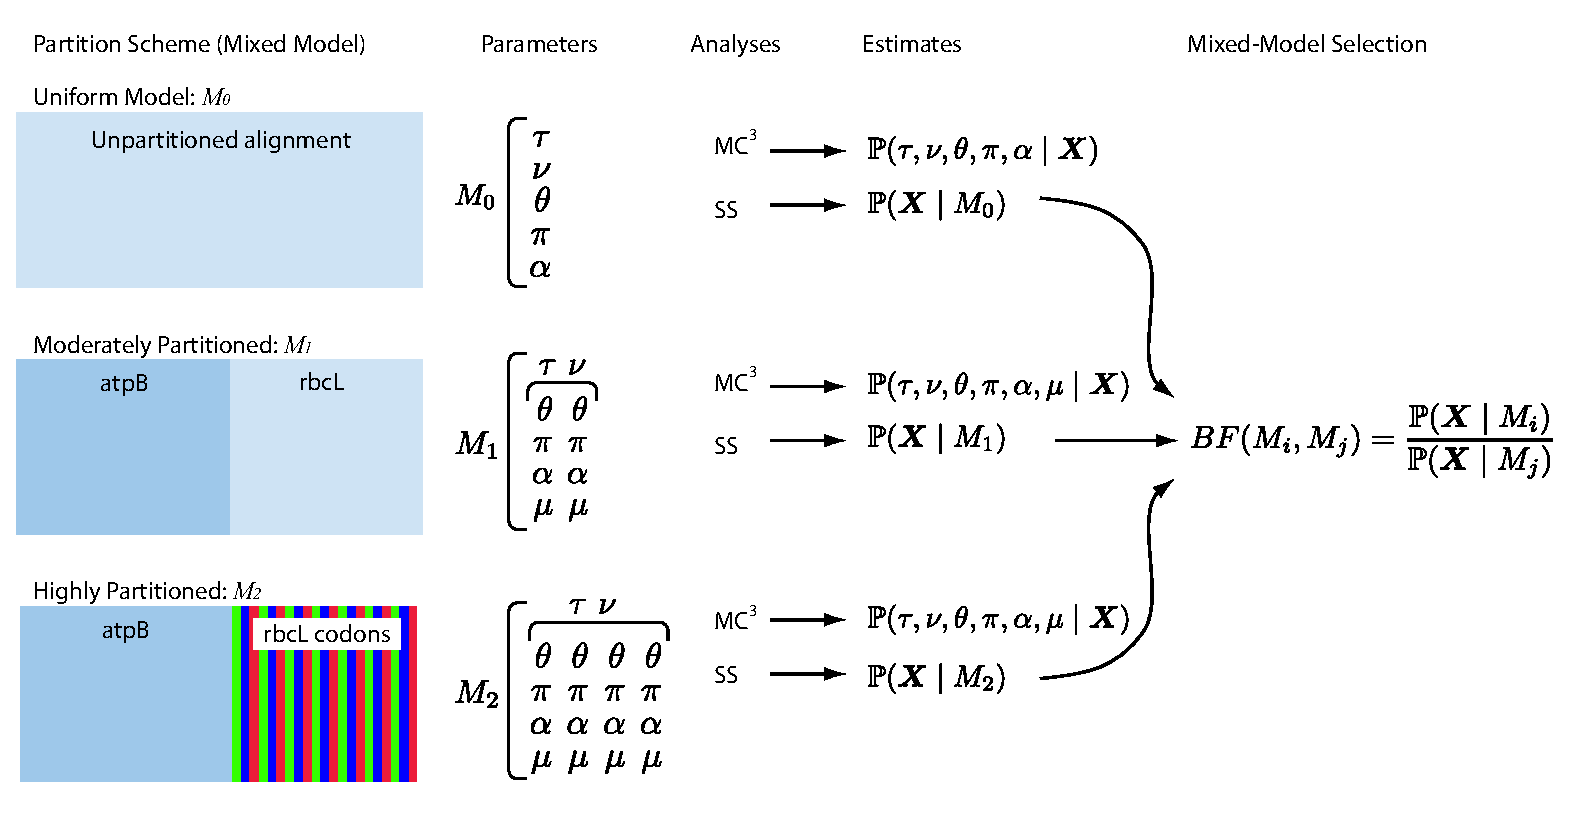
\includegraphics[width=6.8in,angle=0]{figures/pipeline.eps}}
\caption{\small The analysis pipeline for Exercise 1. We will explore three partition schemes for the conifer dataset.
The first model (the `uniform model', $M_0$) assumes that all sites evolved under a common GTR+$\Gamma$ substitution model.
The second model (the `moderately partitioned' model, $M_1$) invokes two data partitions corresponding to the two gene regions (atpB and rbcL), and assumes each subset of sites evolved under an independent GTR+$\Gamma$ model, each with its own rate multiplier, $\mu$.
The final mixed model (the `highly partitioned' model, $M_2$) invokes four data partitions---the first partition corresponds to the atpB gene region, and the remaining partitions correspond to the three codon positons of the rbcL gene region---and each data partition is assumed evolved under an independent GTR+$\Gamma$ substitution model.
Note that we assume that all sites share a common tree topology, $\tau$, and branch-length proportions, $\nu$, for each of the candidate partition schemes.
We perform two separate sets of analyses for each mixed model---a Metropolis-coupled MCMC simulation to approximate the joint posterior probability density of the mixed-model parameters, and a `stepping-stone' MCMC simulation to approximate the marginal likelihood for each mixed model.
The resulting marginal-likelihood estimates are then evaluated using Bayes factors to assess the fit of the data to the three candidate mixed models.  
}
\label{pipeline}
\end{figure}
 
Given two models, $M_0$ and $M_1$, the Bayes factor comparison assessing the relative plausibility of each model as an explanation of the data, $BF(M_0,M_1)$, is:
$$BF(M_0,M_1) = \frac{\mbox{posterior odds}}{\mbox{prior odds}}.$$
The posterior odds is the posterior probability of $M_0$ given the data, $\mathbf X$, divided by the posterior odds of $M_1$ given the data:
$$\mbox{posterior odds} = \frac{\mathbb{P}(M_0 \mid \mathbf X)}{\mathbb{P}(M_1 \mid \mathbf X)},$$
and the prior odds is the prior probability of $M_0$ divided by the prior probability of $M_1$:
$$\mbox{prior odds} = \frac{\mathbb{P}(M_0)}{\mathbb{P}(M_1)}.$$
Thus, the Bayes factor measures the degree to which the data alter our belief regarding the support for $M_0$ relative to $M_1$ \citep{lavine1999bayes}:
\begin{align}\label{BFeq1}
BF(M_0,M_1) = \frac{\mathbb{P}(M_0 \mid \mathbf X, \theta_0)}{\mathbb{P}(M_1 \mid \mathbf X, \theta_1)} \div \frac{\mathbb{P}(M_0)}{\mathbb{P}(M_1)}. 
\end{align}
This, somewhat vague, definition does not lead to clear-cut identification of the ``best'' model. Instead, you must decide the degree of your belief in $M_0$ relative to $M_1$. 
Despite the absence of any strict ``rule-of-thumb'', you can refer to the scale \citep[outlined by][]{jeffreys61} for interpreting these measures (Table \ref{bftable}).
\begin{table}[h]
\centering
\caption{\small The scale for interpreting Bayes factors by Harold \citet{jeffreys61}.} 
\label{bftable}
\begin{tabular}{l c r}
\hline
\multicolumn{1}{l}{\textbf{$BF(M_0, M_1)$}} & \multicolumn{1}{r}{ } &\multicolumn{1}{r}{{Strength of evidence}} \\ 
\hline
$<1:1$ & \hspace{8mm} & Negative (supports $M_1$)\\
$1:1$ to $3:1$ & & Barely worth mentioning\\
$3:1$ to $10:1$ & & Substantial\\
$10:1$ to $30:1$ & & Strong\\
$30:1$ to $100:1$ & & Very strong\\
$>100:1$ & & Decisive\\
\hline
\multicolumn{3}{l}{{\scriptsize{For a detailed description of Bayes factors see \citet{kass95}}}} 
\end{tabular}
\end{table}


Unfortunately, direct calculation of the posterior odds to prior odds ratio is unfeasible for most phylogenetic models. However, we can further define the posterior odds ratio as:
\begin{align*}
\frac{\mathbb{P}(M_0 \mid \mathbf X)}{\mathbb{P}(M_1 \mid \mathbf X)} = \frac{\mathbb{P}(M_0)}{\mathbb{P}(M_1)} \frac{\mathbb{P}(\mathbf X \mid M_0)}{\mathbb{P}(\mathbf X \mid M_1)},
\end{align*}
where $\mathbb{P}(\mathbf X \mid M_i)$ is the \textit{marginal likelihood} of the data marginalized over all parameters for $M_i$; it is also referred to as the \textit{model evidence} or \textit{integrated likelihood}.
More explicitly, the marginal likelihood is the probability of the set of observed data ($\mathbf X$) under a given model ($M_i$), while averaging over all possible values of the parameters of the model ($\theta_i$) with respect to the prior density on $\theta_i$
\begin{align}\label{margeLike}
\mathbb{P}(\mathbf X \mid M_i) = \int \mathbb{P}(\mathbf X \mid \theta_i) \mathbb{P}(\theta_i)dt.
\end{align}
If you refer back to equation \ref{BFeq1}, you can see that, with very little algebra, the ratio of marginal likelihoods is equal to the Bayes factor:
\begin{align}\label{bfFormula}
BF(M_0,M_1) = \frac{\mathbb{P}(\mathbf X \mid M_0)}{\mathbb{P}(\mathbf X \mid M_1)} = \frac{\mathbb{P}(M_0 \mid \mathbf X, \theta_0)}{\mathbb{P}(M_1 \mid \mathbf X, \theta_1)} \div \frac{\mathbb{P}(M_0)}{\mathbb{P}(M_1)}. 
\end{align}
Therefore, we can perform a Bayes factor comparison of two models by calculating the marginal likelihood for each one. % Simple as pie, right?
Alas, exact solutions for calculating marginal likelihoods are not known for phylogenetic models (see equation \ref{margeLike}), thus we must resort to numerical integration methods to estimate or approximate these values. 
In this exercise, we will estimate the marginal likelihood for each partition scheme
using both the harmonic-mean (unreliable) and stepping-stone (preferable) estimators.


\exs{Open the file \cl{conifer\_dna.nex} in your text editor. This file contains the sequences for 2 different genes sampled from 9 species (Box 1). The elements of the \cl{DATA} block indicate the type of data, number of taxa, and length of the sequences.}

\begin{center}
\texttt{\scriptsize
\fbox{
\begin{minipage}{6in}
\begin{tabbing}
\#NEX\=US\\
BEGIN DATA;\\
\>DIMENSIONS NTAX=9 NCHAR=2659;\\
\>FORMAT DATATYPE = DNA GAP = - MISSING = ? INTERLEAVE;\\
\>MATRIX\\
$[$ATPB$]$\\
\>Ginkgo\_biloba\ \ \ \ \ \ \ \ \ \ \ \ \ \ TTATTGGTCCAGTACTGGATGTAGCTTTTCCCCCGGG...\\
\>Araucaria\_araucana\ \ \ \ \ \ \ \ \ -----GGTCCGGTACTGGATGTATCTTTTCCTCCAGA...\\
\>Cedrus\_deodara\ \ \ \ \ \ \ \ \ \ \ \ \ TCATTGGCCCAGTACTGGA?GTCTCTTTTCCTCCAGG...\\
\>Cupressus\_arizonica\ \ \ \ \ \ \ \ -----------------GATGTATCTTTCCCTCCAGG...\\
\>Juniperus\_communis\ \ \ \ \ \ \ \ \ -------------------------------------...\\
\>Pinus\_densiflora\ \ \ \ \ \ \ \ \ \ \ TCATTGGCCCAGTACTGGATGTCTCTTTTCCTCCAGG...\\
\>Podocarpus\_chinensis\ \ \ \ \ \ \ TCATCGGCCCTGTACTGGATGTATCTTTTCCTCCAGA...\\
\>Sciadopitys\_verticillata\ \ \ TCATTGGTCCAGTACTAGATGTATCTTTCCCTCCAGG...\\
\>Taxus\_baccata\ \ \ \ \ \ \ \ \ \ \ \ \ \ TTATCGGCCCAGTACTAGATGTCTCTTTTCCTCCAGG...\\
\\
$[$RBCL$]$\\
\>Ginkgo\_biloba\ \ \ \ \ \ \ \ \ \ \ \ \ \ \ \ ATGGATAAGTT------------------AAAGAG...\\
\>Araucaria\_araucana\ \ \ \ \ \ \ \ \ \ \ ATAGATTAACTACTCCGCAATATCAGACCAAAGAT...\\
\>Cedrus\_deodara\ \ \ \ \ \ \ \ \ \ \ \ \ \ \ ACAGATTAACTACTCCTGAATATCAGACCAAAGAT...\\
\>Cupressus\_arizonica\ \ \ \ \ \ \ \ \ \ ----ATTAACTACTCCGGAATATCAGACCAAAGAT...\\
\>Juniperus\_communis\ \ \ \ \ \ \ \ \ \ \ ACAGATTAACTACTCCGGAATATCAGACAAAAGAT...\\
\>Pinus\_densiflora\ \ \ \ \ \ \ \ \ \ \ \ \ ACAGATTAACTACTCCTGAATATCAGACCAAAGAT...\\
\>Podocarpus\_chinensis\ \ \ \ \ \ \ \ \ ACAGATTAACTACTCCGGAATATCAGACCAAAGAT...\\
\>Sciadopitys\_verticillata\ \ \ \ \ ACAGATTAACTACCCCTGAATATCAGACCAAAGAC...\\
\>Taxus\_baccata\ \ \ \ \ \ \ \ \ \ \ \ \ \ \ \ ACAGACTAACTACTCCACAATATCAGACCAAAGAT...\\
;\\
END;\\
\end{tabbing}
\end{minipage}
}}
\vspace{3mm}\\
Box 1: A fragment of the NEXUS file containing the sequences for this exercise. \\
\end{center}

\exs{Open the Rev file, \taha{Rev file name}, in a text editor.  This file contains 
all of the commands required to perform the necessary analyses to explore various
partition schemes (unpartitioned, partitioned by gene region, and partitioned by
gene region$+$codon position).  The details of each command are described in adjacent comments, after a \cl{\#}; {\it e.g.}, \cl{\# this is a Rev comment}. }

Typically, we would perform these analyses by simply sourcing this file in RevBayes. For the purposes of this exercise, however, we will walk through the different steps interactively in the command line.

\bigskip
\subsubsection*{Launch RevBayes}

Execute the RevBayes binary. If this program is in your path, then you can simply type in your Unix terminal:

\exs{\cl{> rb}}

When you execute the program, you will see the program information, including the current version number and functions that will provide information about the program --- \cl{contributors()} and \cl{license()}.% --- and a command reference \cl{help}. 
Execute the \cl{help()} function by typing:

{\tt \begin{snugshade*}
\begin{lstlisting}
RevBayes > help()
\end{lstlisting}
\end{snugshade*}}
\taha{will there be help information by this time?}

This displays a list of the different elements and commands available in RevBayes. The \cl{help} command also provides more detailed information about each of these items.

For example, we can view the \cl{help()} information about the \cl{log()} function:

{\tt \begin{snugshade*}
\begin{lstlisting}
RevBayes > help(log)
\end{lstlisting}
\end{snugshade*}}

\taha{This doesn't do anything}

The \cl{log()} function computes the \cl{base} logarithm of a positive number \cl{x}. \taha{maybe say something about types, e.g., RealPos}

Additionally, RevBayes will print the correct usage of a function if it is executed without any arguments:
{\tt \begin{snugshade*}
\begin{lstlisting}
RevBayes > log()
     Error:    Argument mismatch for call to function `log'( ). 
     Correct usage is: Real function (RealPos x, RealPos base)
\end{lstlisting}
\end{snugshade*}}

%allows you to save all of the screen output from your analysis to a log file. 
%The \cl{help} information for this command displays all of the available options for specifying screen logging.
%We are going to log our screen output to a file called \cl{conifer-partn-log.txt}.
%\mbcl{log start filename=conifer-partn-log.txt}
%
%Next, load the sequences into the program using the \cl{execute} command.
%\mbcl{execute conifer\_dna.nex}

%\bigskip
%\subsubsection*{Load the Sequences}% \& Specify the Outgroup}



\bigskip
\subsection{An Unpartitioned Analysis}\label{secUnif} 

\textbf{\textit{Load Data}}

First load in the sequences using the \cl{readCharacterData} function:

{\tt \begin{snugshade*}
\begin{lstlisting}
RevBayes > D <- readCharacterData("data/conifer_atpB.nex")
RevBayes > data_atpB <- D[1]
RevBayes > D <- readCharacterData("data/conifer_rbcL.nex")
RevBayes > data_rbcL <- D[1]
\end{lstlisting}
\end{snugshade*}}

\taha{Concatenate two datasets}

{\tt \begin{snugshade*}
\begin{lstlisting}
RevBayes > data <- data_atpB + data_rbcL
\end{lstlisting}
\end{snugshade*}}

{\tt \begin{snugshade*}
\begin{lstlisting}
RevBayes > data
   Origination:                   conifer_atpB.nex
   Number of taxa:                9
   Number of characters:          2659
   Number of included characters: 2659
   Datatype:                      DNA
\end{lstlisting}
\end{snugshade*}}

\taha{can we specify an outgroup?}

%Now that RevBayes has read in our data, we can define our outgroup taxon. Unless a clock-based analysis is specified, MrBayes v3.2 infers {\em unrooted} trees, however trees are written to output files as rooted trees (unrooted trees are not phylogenies as they do not specify a temporal direction). 
%Accordingly, this command specifies how we would like our trees written to file.
%If we do not specify an outgroup, the trees will be rooted on the first species in the data matrix by default. 
%\mbcl{outgroup Ginkgo\_biloba}

Next we will specify some useful variables based on our dataset. The variable \cl{data} has \textsl{member functions} that we can use to retrieve information. 
{\tt \begin{snugshade*}
\begin{lstlisting}
RevBayes > n_species <- data.ntaxa()
RevBayes > n_sites <- data.nchar()[1]
RevBayes > names <- data.names()
RevBayes > n_nodes <- 2 * n_species - 3
\end{lstlisting}
\end{snugshade*}}

\textbf{\textit{The GTR Parameters}}

The first analysis in this exercise involves performing an analysis on our unpartitioned alignment. 
This corresponds to the assumption that the process that gave rise to our data was homogeneous across all sites of the alignment. 
Specifically, we will assume that both genes evolved under the same GTR$+\Gamma$ model (Fig.~\ref{pipeline}). 

\taha{describe setting up model and some background on GTR...}

%The \cl{lset} command is used to specify the details of our sequence model. 
%\mbcl{lset nst=6 rates=gamma}

%This command specifies a substitution matrix with six relative substitution rates (GTR) with gamma-distributed rate variation across sites. 
%Because models are specified this way, it is apparent that some types of DNA models are not available in MrBayes. Thus, with the \cl{nst} element of the \cl{lset} command, we can specify the JC69 or F81 models (\cl{nst=1}), the K2P or HKY models (\cl{nst=2}), or the GTR model (\cl{nst=6}).
%
%The Bayesian perspective views parameters as random variables, which requires that we specify a prior probability density that describes the precise nature of that random variation. 
%Accordingly, we need to specify priors for all of the parameters of the specified nucleotide substitution model. 
%The command for modifying priors is the \cl{prset} command. 
%
%Use the \cl{help} command to view the list of priors available for modification:
%
%\mbcl{help prset}

First, we will define and specify a prior on the exchangeability rates of the GTR model. We will use a flat Dirichlet prior on these six rates. To do this, we must begin by defining a constant node that specifies the vector of concentration values of the Dirichlet prior using the \cl{v()} function:
{\tt \begin{snugshade*}
\begin{lstlisting}
RevBayes > er_prior <- v(1,1,1,1,1,1) 
\end{lstlisting}
\end{snugshade*}}

The constant variable \cl{er\_prior} defines the parameters of the Dirichlet prior distribution on the exchangeability rates. Thus, we can create a stochastic node for the exchangeability rates using the \cl{dnDirichlet()} function, which takes a vector of values as an argument and the \cl{\rbdn} operator. Together, these create a stochastic node named ``\cl{er}'': 

{\tt \begin{snugshade*}
\begin{lstlisting}
RevBayes > er ~ dnDirichlet(er_prior)
\end{lstlisting}
\end{snugshade*}}

The Dirichlet distribution assigns probability densities to grouped parameters: {\it e.g.}, those that measure proportions and must sum to 1. 
Above, we specified a 6-parameter Dirichlet prior on the relative rates of the GTR model, where the placement of each value specified represents one of the 6 relative rates: (1) $A\leftrightarrows C$, (2) $A\leftrightarrows G$, (3) $A\leftrightarrows T$, (4) $C\leftrightarrows G$, (5) $C\leftrightarrows T$, (6) $G\leftrightarrows T$. 
The input parameters of a Dirichlet distribution are called shape parameters or concentration parameters and a value is specified for each of the 6 GTR rates. 
The expectation and variance for each variable are related to the sum of the shape parameters.
The prior above is a `flat' or symmetric Dirichlet since all of the shape parameters are equal (1,1,1,1,1,1), thus we are specifying a model that allows for equal rates of change between nucleotides, such that the expected rate for each is equal to $\frac{1}{6}$ \citep{zwickl04}.
Figure \ref{dirichletFig}a shows the probability density of each rate under this model.
If we parameterized the Dirichlet distribution such that all of the parameters were equal to 100, this would also specify a prior with an expectation of equal exchangeability rates (Figure \ref{dirichletFig}b). 
However, by increasing the shape parameters of the Dirichlet distribution, \cl{er\_prior <- v(100,100,100,100,100,100)}, would heavily restrict the MCMC from sampling sets of GTR rates in which the values were not equal or very nearly equal ({\it i.e.}, this is a very {\em informative} prior). 
We can consider a different Dirichlet parameterization if we had strong prior belief that transitions and transversions occurred at different rates.
In this case, we could specify a more informative prior density: \cl{er\_prior <- v(4,8,4,4,8,4)}. 
Under this model, the expected rate for transversions would be $\frac{4}{32}$ and the expected rate for transitions would equal $\frac{8}{32}$, and there would be greater prior probability on sets of GTR rates that matched this configuration (Figure \ref{dirichletFig}c). 
An alternative informative prior would be one where we assumed that each of the 6 GTR rates had a different value conforming to a Dirichlet(2,4,6,8,10,12). 
This would lead to a different prior probability density for each rate parameter (Figure \ref{dirichletFig}d).
Without strong prior knowledge about the pattern of relative rates, however, we can better capture our statistical uncertainty with a vague prior on the GTR rates. 
Notably, all patterns of relative rates have the same probability under \cl{er\_prior <- v(1,1,1,1,1,1)}.
\begin{figure}[h]
\centering
\fbox{\includegraphics[width=5in,angle=-90]{figures/dirichlet_rates.eps}}
\caption{\small Four different examples of Dirichlet priors on exchangeability rates.}
\label{dirichletFig}
\end{figure}

\taha{implement the move for each stocastic parameter at the same time...}

For each stochastic node in our model, we must also specify a proposal mechanism if we wish to sample that value. 
The Dirichlet prior on our parameter \cl{er} creates a \href{http://en.wikipedia.org/wiki/Simplex}{\textit{simplex}} of values that sum to 1. 
In RevBayes, there are many different proposal mechanisms --- called ``moves'' --- and each move operates on a specific data type. \taha{more here...}

Check the value type of the variable \cl{er} using the \cl{structure()} function:

{\tt \begin{snugshade*}
\begin{lstlisting}
RevBayes > structure(er)

   _valueType    = Vector<RealPos>
   _objectType   = Container
   _value        = [ 1, 1, 1, 1, 1, 1 ]
\end{lstlisting}
\end{snugshade*}}

All moves go in a vector...instantiate the first element of our vector of moves by setting the proposal on the exchangeability rates:

{\tt\small \begin{snugshade*}
\begin{lstlisting}
RevBayes > moves[1] <- mvSimplexElementScale(er, alpha=10, tune=true, weight=3) 
\end{lstlisting}
\end{snugshade*}}



We can use the same type of distribution as a prior on the 4 base frequencies ($\pi_A, \pi_C, \pi_G, \pi_T$) since these parameters also represent proportions. 
Specify a flat Dirichlet prior density on the base frequencies:

{\tt \begin{snugshade*}
\begin{lstlisting}
RevBayes > sf_prior <- v(1,1,1,1) 
RevBayes > sf ~ dnDirichlet(sf_prior)
\end{lstlisting}
\end{snugshade*}}

And specify the simplex scale move:
{\tt \small \begin{snugshade*}
\begin{lstlisting}
RevBayes > moves[2] <- mvSimplexElementScale(sf, alpha=10, tune=true, weight=2)  
\end{lstlisting}
\end{snugshade*}}

\taha{Now say something about the instantaneous rate matrix here and deterministic nodes}

{\tt \begin{snugshade*}
\begin{lstlisting}
RevBayes > Q := gtr(er,sf)
\end{lstlisting}
\end{snugshade*}}


\textbf{\textit{Gamma-Distributed Site Rates}}

We will also assume that the substitution rates vary among sites according to a gamma distribution, which has two parameters: the shape parameter, $\alpha$, and the scale parameter, $\beta$. 
In order that we can interpret the branch lengths as the expected number of substitutions per site, this model assumes that the mean site rate is equal to 1.
%Consequently, we wish to specify a gamma distribution with a mean of 1.
The mean of the gamma is equal to $\alpha/\beta$, so a mean-one gamma is specified by setting the two parameters to be equal, $\alpha=\beta$.
Therefore, we need only consider the single shape parameter, $\alpha$ \citep{yang94a}. 
The degree of among-site substitution rate variation (ASRV) is inversely proportional to the value of the shape parameter---as the value of $\alpha$-shape parameter increases, the gamma distribution increasingly resembles a normal distribution with decreasing variance, which corresponds to decreasing levels of ASRV (Figure \ref{asrhGammaFig}).
If $\alpha = 1$, then the gamma distribution collapses to an exponential distribution with a rate parameter equal to $\beta$.
By contrast, when the value of the $\alpha$-shape parameter is $< 1$, the gamma distribution assumes a concave distribution that places most of the prior density on low rates but allows some prior mass on sites with very high rates, which corresponds to high levels of ASRV (Figure \ref{asrhGammaFig}).

Alternatively, we might not have good prior knowledge about the variance in site rates, thus we can place an uninformative, or diffuse prior on the shape parameter.
For this analysis, we will use an exponential distribution with a rate parameter, \cl{shape\_prior}, equal to \cl{0.05}.
Under an exponential prior, we are placing non-zero probability on values of $\alpha$ ranging from 0 to $\infty$. 
The rate parameter, often denoted $\lambda$, of an exponential distribution controls both the mean and variance of this prior such that the expected (or mean) value of $\alpha$ is:
$$\mathbb{E}[\alpha] = \frac{1}{\lambda}.$$
Thus, if we set $\lambda=0.05$, then $\mathbb{E}[\alpha] = 20$.
%The gamma shape parameter is called \cl{shapepr} in the \cl{prset} command.

{\tt\begin{snugshade*}
\begin{lstlisting}
RevBayes > shape_prior <- 0.05                                                                             
RevBayes > shape ~ dnExponential(shape_prior)
\end{lstlisting}
\end{snugshade*}}

\taha{write something about setting up and normalizing gamma rates...}
{\tt \begin{snugshade*}
\begin{lstlisting}
RevBayes > norm_gamma_rates := discretizeGamma( shape, 4 )
\end{lstlisting}
\end{snugshade*}}



\begin{figure}[h]
\centering
\fbox{\includegraphics[width=3in,angle=-90]{figures/asrh_gamma.eps}}
\caption{\small The probability density of mean-one gamma-distributed rates under different shape parameters.}
\label{asrhGammaFig}
\end{figure}

The random variable that controls the rate variation is the stochastic node \cl{shape}. This variable is a single, real positive value (\cl{RealPos} datatype in RevBayes). 
Thus, we will apply a simple scale move to this parameter:

{\tt \begin{snugshade*}
\begin{lstlisting}
moves[3] <- mvScale(shape, lambda=1.0, tune=true, weight=1.0)\end{lstlisting}
\end{snugshade*}}


\textbf{\textit{Tree Topology and Branch Lengths}}

{\tt \begin{snugshade*}
\begin{lstlisting}
RevBayes > topology ~ uniformTopology(n_species, names)
\end{lstlisting}
\end{snugshade*}}

{\tt \begin{snugshade*}
\begin{lstlisting}
RevBayes > moves[4] <- mvNNI(topology, weight=5.0)
\end{lstlisting}
\end{snugshade*}}

{\tt \small \begin{snugshade*}
\begin{lstlisting}
RevBayes > for (i in 1:n_branches) {
RevBayes +  br_lens[i] ~ dnExponential(1.0)
RevBayes +  moves[i+4] <- mvScale(br_lens[i],lambda=1,tune=true,weight=1) 
RevBayes + }
\end{lstlisting}
\end{snugshade*}}

{\tt \begin{snugshade*}
\begin{lstlisting}
RevBayes > phylogeny := treeAssembly(topology, br_lens)
\end{lstlisting}
\end{snugshade*}}




\textbf{\textit{Putting it All Together}}

{\tt \begin{snugshade*}
\begin{lstlisting}
RevBayes > phyloSeq ~ phyloCTMC(tree=phylogeny, Q=Q, siteRates=norm_gamma_rates, nSites=n_sites, type="DNA")
\end{lstlisting}
\end{snugshade*}}

{\tt \begin{snugshade*}
\begin{lstlisting}
RevBayes > phyloSeq.clamp(data)
\end{lstlisting}
\end{snugshade*}}

{\tt \begin{snugshade*}
\begin{lstlisting}
RevBayes > mymodel <- model(sf)
\end{lstlisting}
\end{snugshade*}}

Now we have specified a simple, single-partition analysis---each parameter of the model will be estimated from every site in our alignment.

\taha{list all in model}
{\tt \begin{snugshade*}
\begin{lstlisting}
RevBayes > mymodel
\end{lstlisting}
\end{snugshade*}}


\subsubsection*{Calculating the Marginal Likelihood}

{\tt \begin{snugshade*}
\begin{lstlisting}
RevBayes > pow_p <- powerPosterior(mymodel, moves, "pow_p_uniform.out", cats=50) 
\end{lstlisting}
\end{snugshade*}}

{\tt \begin{snugshade*}
\begin{lstlisting}
RevBayes > pow_p.burnin(generations=1000,tuningInterval=100)
\end{lstlisting}
\end{snugshade*}}

{\tt \begin{snugshade*}
\begin{lstlisting}
RevBayes > pow_p.run(generations=1000)  
\end{lstlisting}
\end{snugshade*}}

{\tt \small \begin{snugshade*}
\begin{lstlisting}
RevBayes > ss <- steppingStoneSampler(file="pow_posterior_uniform.out", powerColumnName="power", likelihoodColumnName="likelihood")
\end{lstlisting}
\end{snugshade*}}

Compute the marginal likelihood under stepping-stone sampling using the member function \cl{marginal()} of the \cl{ss} variable and record the value in table \ref{ssTable}.
{\tt \begin{snugshade*}
\begin{lstlisting}
RevBayes > ss.marginal() 
\end{lstlisting}
\end{snugshade*}}


{\tt \small \begin{snugshade*}
\begin{lstlisting}
RevBayes > ps <- pathSampler(file="pow_posterior_uniform.out", powerColumnName="power", likelihoodColumnName="likelihood")
\end{lstlisting}
\end{snugshade*}}

{\tt \begin{snugshade*}
\begin{lstlisting}
RevBayes > ps.marginal() 
\end{lstlisting}
\end{snugshade*}}





%%%%%%%%



\bigskip
\subsection{Partitioning by Gene Region}\label{secByGene}

The uniform model used in the previous section assumes that all sites in the alignment evolved under the same process described by a shared tree, branch length proportions, and parameters of the GTR+$\Gamma$ substitution model.
However, our alignment contains two distinct gene regions---atpB and rbcL---so we may wish to explore the possibility that the substitution process differs between these two gene regions.
This requires that we first specify the data partitions corresponding to these two genes, then define an independent substitution model for each data partition. 

\textbf{\textit{Clear Workspace and Reload Data}}

\taha{this time reading from 2 different files}

{\tt \begin{snugshade*}
\begin{lstlisting}
RevBayes > clear()
\end{lstlisting}
\end{snugshade*}}

{\tt \begin{snugshade*}
\begin{lstlisting}
RevBayes > filenames <- v("data/conifer_atpb.nex", "data/conifer_rbcL.nex")
\end{lstlisting}
\end{snugshade*}}

{\tt \begin{snugshade*}
\begin{lstlisting}
RevBayes > n_parts <- filenames.size()
\end{lstlisting}
\end{snugshade*}}

{\tt \begin{snugshade*}
\begin{lstlisting}
RevBayes > for (i in 1:n_parts){
RevBayes +    data[i] <- readCharacterData(filenames[i])[1]
RevBayes + }
\end{lstlisting}
\end{snugshade*}}

{\tt \begin{snugshade*}
\begin{lstlisting}
RevBayes > n_species <- data[1].ntaxa()
RevBayes > names <- data[1].names()
RevBayes > n_branches <- 2 * n_species - 3
\end{lstlisting}
\end{snugshade*}}

\textbf{\textit{Specify the Parameters by Looping Over Partitions}}


{\tt \small \begin{snugshade*}
\begin{lstlisting}
mv_it <- 0
for (i in 1:n_parts){
  ## index i=1 : atpB gene
  ## index i=2 : rbcL gene

  # Exchangeability rates #
  er_prior[i] <- v(1,1,1,1,1,1)
  er[i] ~ dnDirichlet(er_prior[i])
  moves[mv_it++] <- mvSimplexElementScale(er[i], alpha=10, tune=true, weight=3) 

  # Stationary frequencies #
  sf_prior[i] <- v(1,1,1,1)
  sf[i] ~ dnDirichlet(sf_prior[i])
  moves[mv_it++] <- mvSimplexElementScale(sf[i], alpha=10, tune=true, weight=2) 

  # GTR Rate Matrix (deterministic node) #
  Q[i] := gtr(er[i],sf[i]) 

  # Gamma-dist site rates #
  shape_prior[i] <- 0.05 
  shape[i] ~ dnExponential( shape_prior[i] )
  norm_gamma_rates[i] := discretizeGamma( shape[i], 4 )
  moves[mv_it++] <- mvScale(shape[i], lambda=1.0, tune=true, weight=1.0)
}
\end{lstlisting}
\end{snugshade*}}


\textbf{\textit{Uniform Topology and Branch Lengths}}

{\tt \begin{snugshade*}
\begin{lstlisting}
# Uniform Topology #
topology ~ uniformTopology(n_species, names)
moves[mv_it++] <- mvNNI(topology, weight=1.0)

# Branch lengths #
for (i in 1:n_branches) {
  br_lens[i] ~ exponential(1.0)
  moves[mv_it++] <- mvScale(br_lens[i],lambda=1,tune=true,weight=1) 
}

# Create the phylogeny by combining topology & branch lengths #
phylogeny := treeAssembly(topology, br_lens)
\end{lstlisting}
\end{snugshade*}}

\textbf{\textit{Putting it All Together}}

{\tt \begin{snugshade*}
\begin{lstlisting}
for (i in 1:n_parts){
  phyloSeq[i] ~ phyloCTMC(tree=phylogeny, Q=Q[i], siteRates=norm_gamma_rates[i], nSites=data[i].nchar()[1], type="DNA")
  phyloSeq[i].clamp(data[i])
}
\end{lstlisting}
\end{snugshade*}}


{\tt \begin{snugshade*}
\begin{lstlisting}
RevBayes > mymodel <- model(topology)
\end{lstlisting}
\end{snugshade*}}

\subsubsection*{Calculating the Marginal Likelihood}

{\tt \begin{snugshade*}
\begin{lstlisting}
RevBayes > pow_p <- powerPosterior(mymodel, moves, file="pow_posterior_twogene.out", cats=50) 
RevBayes > pow_p.burnin(generations=1000,tuningInterval=100)
RevBayes > pow_p.run(generations=1000)  
\end{lstlisting}
\end{snugshade*}}

{\tt \begin{snugshade*}
\begin{lstlisting}
RevBayes > ss <- steppingStoneSampler(file="pow_posterior_twogene.out", powerColumnName="power", likelihoodColumnName="likelihood")
RevBayes > ss.marginal() 
\end{lstlisting}
\end{snugshade*}}

{\tt \begin{snugshade*}
\begin{lstlisting}
RevBayes > ps <- pathSampler(file="pow_posterior_twogene.out", powerColumnName="power", likelihoodColumnName="likelihood")
RevBayes > ps.marginal() 
\end{lstlisting}
\end{snugshade*}}




\bigskip
\subsection{Partitioning by Codon Position and by Gene}\label{secExtremeP}

Because of the genetic code, we often find that different positions within a codon (first, second, and third) evolve at different rates.
Thus, using our knowledge of biological data, we can devise a third approach that further partitions our alignment. 
For this exercise, we will partition sites within the rbcL gene by codon position.

\textbf{\textit{Clear Workspace and Reload Data}}

{\tt \begin{snugshade*}
\begin{lstlisting}
RevBayes > clear()
RevBayes > data[1] <- readCharacterData("data/conifer_atpB.nex")[1]
RevBayes > data_rbcL <- readCharacterData("data/conifer_rbcL.nex")[1]
\end{lstlisting}
\end{snugshade*}}

\textbf{\textit{Specify Data Matrices for Each Codon Position}}

{\tt \begin{snugshade*}
\begin{lstlisting}
RevBayes > n_sites_rbcL <- data_rbcL.nchar()[1]
RevBayes > vec_1pos <- seq(1,n_sites_rbcL,3)
RevBayes > vec_2pos <- seq(2,n_sites_rbcL,3)
RevBayes > vec_3pos <- seq(3,n_sites_rbcL,3)
\end{lstlisting}
\end{snugshade*}}

\taha{assign the rbcL data to the vector of data matrices}
{\tt \begin{snugshade*}
\begin{lstlisting}
RevBayes > data[2] <- data_rbcL	# codon position 1
RevBayes > data[3] <- data_rbcL	# codon position 2
RevBayes > data[4] <- data_rbcL	# codon position 3
\end{lstlisting}
\end{snugshade*}}

{\tt \begin{snugshade*}
\begin{lstlisting}
RevBayes > for(i in vec_1pos){
RevBayes +    data[3].excludeCharacter(i) 
RevBayes +    data[4].excludeCharacter(i)
RevBayes + }
\end{lstlisting}
\end{snugshade*}}

{\tt \begin{snugshade*}
\begin{lstlisting}
RevBayes > for(i in vec_2pos){
RevBayes +    data[2].excludeCharacter(i) 
RevBayes +    data[4].excludeCharacter(i)
RevBayes + }
\end{lstlisting}
\end{snugshade*}}

{\tt \begin{snugshade*}
\begin{lstlisting}
RevBayes > for(i in vec_3pos){
RevBayes +    data[2].excludeCharacter(i) 
RevBayes +    data[3].excludeCharacter(i)
RevBayes + }
\end{lstlisting}
\end{snugshade*}}

\taha{create a vector of dataset sizes}
{\tt \begin{snugshade*}
\begin{lstlisting}
RevBayes > n_sites[1] <- data[1].nchar()[1]
RevBayes > n_sites[2] <- vec_1pos.size()
RevBayes > n_sites[3] <- vec_2pos.size()
RevBayes > n_sites[4] <- vec_3pos.size()
\end{lstlisting}
\end{snugshade*}}

{\tt \begin{snugshade*}
\begin{lstlisting}
RevBayes > n_parts <- data.size()
\end{lstlisting}
\end{snugshade*}}

{\tt \begin{snugshade*}
\begin{lstlisting}
RevBayes > n_species <- data[1].ntaxa()
RevBayes > names <- data[1].names()
RevBayes > n_branches <- 2 * n_species - 3
\end{lstlisting}
\end{snugshade*}}



\textbf{\textit{Specify the Parameters by Looping Over Partitions}}


{\tt \small \begin{snugshade*}
\begin{lstlisting}
mv_it <- 0
for (i in 1:n_parts){
  ## index i=1 : atpB gene
  ## index i=2 : rbcL gene position 1
  ## index i=3 : rbcL gene position 2
  ## index i=4 : rbcL gene position 3

  # Exchangeability rates #
  er_prior[i] <- v(1,1,1,1,1,1)
  er[i] ~ dnDirichlet(er_prior[i])
  moves[mv_it++] <- mvSimplexElementScale(er[i], alpha=10, tune=true, weight=3) 

  # Stationary frequencies #
  sf_prior[i] <- v(1,1,1,1)
  sf[i] ~ dnDirichlet(sf_prior[i])
  moves[mv_it++] <- mvSimplexElementScale(sf[i], alpha=10, tune=true, weight=2) 

  # GTR Rate Matrix (deterministic node) #
  Q[i] := gtr(er[i],sf[i]) 

  # Gamma-dist site rates #
  shape_prior[i] <- 0.05 
  shape[i] ~ dnExponential( shape_prior[i] )
  norm_gamma_rates[i] := discretizeGamma( shape[i], 4 )
  moves[mv_it++] <- mvScale(shape[i], lambda=1.0, tune=true, weight=1.0)
}
\end{lstlisting}
\end{snugshade*}}


\textbf{\textit{Uniform Topology and Branch Lengths}}

{\tt \begin{snugshade*}
\begin{lstlisting}
# Uniform Topology #
topology ~ uniformTopology(n_species, names)
moves[mv_it++] <- mvNNI(topology, weight=1.0)

# Branch lengths #
for (i in 1:n_branches) {
  br_lens[i] ~ exponential(1.0)
  moves[mv_it++] <- mvScale(br_lens[i],lambda=1,tune=true,weight=1) 
}

# Create the phylogeny by combining topology & branch lengths #
phylogeny := treeAssembly(topology, br_lens)
\end{lstlisting}
\end{snugshade*}}

\textbf{\textit{Putting it All Together}}

{\tt \begin{snugshade*}
\begin{lstlisting}
for (i in 1:n_parts){
  phyloSeq[i] ~ phyloCTMC(tree=phylogeny, Q=Q[i], siteRates=norm_gamma_rates[i], nSites=data[i].nchar()[1], type="DNA")
  phyloSeq[i].clamp(data[i])
}
\end{lstlisting}
\end{snugshade*}}


{\tt \begin{snugshade*}
\begin{lstlisting}
RevBayes > mymodel <- model(topology)
\end{lstlisting}
\end{snugshade*}}


\subsubsection*{Calculating the Marginal Likelihood}

{\tt \begin{snugshade*}
\begin{lstlisting}
RevBayes > pow_p <- powerPosterior(mymodel, moves, file="pow_posterior_genecodon.out", cats=50) 
RevBayes > pow_p.burnin(generations=1000,tuningInterval=100)
RevBayes > pow_p.run(generations=1000)  
\end{lstlisting}
\end{snugshade*}}

{\tt \begin{snugshade*}
\begin{lstlisting}
RevBayes > ss <- steppingStoneSampler(file="pow_posterior_genecodon.out", powerColumnName="power", likelihoodColumnName="likelihood")
RevBayes > ss.marginal() 
\end{lstlisting}
\end{snugshade*}}

{\tt \begin{snugshade*}
\begin{lstlisting}
RevBayes > ps <- pathSampler(file="pow_posterior_genecodon.out", powerColumnName="power", likelihoodColumnName="likelihood")
RevBayes > ps.marginal() 
\end{lstlisting}
\end{snugshade*}}



\bigskip
\subsection{Compute Bayes Factors and Select Model}


Now that we have estimates of the marginal likelihood under each of our different models, we can evaluate their relative plausibility using Bayes factors.
Use Table \ref{ssTable} to summarize the marginal log-likelihoods estimated using the stepping-stone and path-sampling methods.
\begin{Form}
\begin{table}[h]
\centering
\caption{\small Estimated marginal likelihoods for different partition configurations$^*$.}
\begin{tabular}{l c c c c}
\hline
\multicolumn{1}{l}{\textbf{ }} &\multicolumn{1}{r}{\textbf{ }} & \multicolumn{3}{c}{\textbf{Marginal lnL estimates}} \\ 
\cline{3-5}
\multicolumn{1}{l}{\textbf{Partition}} & \multicolumn{1}{r}{\hspace{3mm}} & \multicolumn{1}{c}{\textit{Stepping-stone}} & \multicolumn{1}{r}{\hspace{3mm}} & \multicolumn{1}{c}{\textit{Path sampling}} \\ 
\hline
\ref{secUnif} uniform ($M_1$) & \hspace{15mm} & \TextField[name=m1,backgroundcolor={.85 .85 .85},color={1 0 0},height=4ex]{}  & \hspace{15mm} & \TextField[name=ml2,backgroundcolor={.85 .85 .85},color={0 0 1},height=4ex]{} \\
\hline
\ref{secByGene} moderate ($M_2$) & \hspace{3mm} &\TextField[name=ml3,backgroundcolor={.85 .85 .85},color={1 0 0},height=4ex]{}   & \hspace{3mm} & \TextField[name=ml4,backgroundcolor={.85 .85 .85},color={0 0 1},height=4ex]{} \\
\hline
\ref{secExtremeP} extreme ($M_3$) & \hspace{3mm} & \TextField[name=ml5,backgroundcolor={.85 .85 .85},color={1 0 0},height=4ex]{} & \hspace{3mm} & \TextField[name=ml6,backgroundcolor={.85 .85 .85},color={0 0 1},height=4ex]{} \\
\hline
{\footnotesize{$^*$you can edit this table}}\\
\end{tabular}
\label{ssTable}
\end{table}
\end{Form}

Phylogenetics software programs log-transform the likelihood to avoid \href{http://en.wikipedia.org/wiki/Arithmetic_underflow}{underflow}, because multiplying likelihoods results in numbers that are too small to be held in computer memory.
Thus, we must use a different form of equation \ref{bfFormula} to calculate the ln-Bayes factor (we will denote this value $\mathcal{K}$):
\begin{align}\label{LNbfFormula}
\mathcal{K}=\ln[BF(M_0,M_1)] = \ln[\mathbb{P}(\mathbf X \mid M_0)]-\ln[\mathbb{P}(\mathbf X \mid M_1)],
\end{align}
where $\ln[\mathbb{P}(\mathbf X \mid M_0)]$ is the \textit{marginal lnL} estimate for model $M_0$. 
The value resulting from equation \ref{LNbfFormula} can be converted to a raw Bayes factor by simply taking the exponent of $\cal{K}$
\begin{align}\label{LNbfFormula2}
BF(M_0,M_1) = e^{\cal{K}}.
\end{align}
Alternatively, you can interpret the strength of evidence in favor of $M_0$ using the $\cal{K}$ and skip equation \ref{LNbfFormula2}. 
In this case, we evaluate the $\cal{K}$ in favor of model $M_0$ against model $M_1$ so that:
\begin{center}
\begin{tabular}{l}
if $\mathcal{K} > 1$, then model $M_0$ wins\\
if $\mathcal{K} < -1$, then model $M_1$ wins.
\end{tabular}
\end{center}
Thus, values of $\mathcal{K}$ around 0 indicate ambiguous support. 

%Alternatively, you can refer to a different scale for interpreting the $\ln[BF(M_0,M_1)]$ described by \citet{kass95}.
%\begin{table}[h]
%\centering
%\caption{\small The scale for interpreting $log_e$ Bayes factors by \citet{kass95}.} 
%\begin{tabular}{l c r}
%\hline
%\multicolumn{1}{l}{\textbf{$2\ln[BF(M_0, M_1)]$}} & \multicolumn{1}{r}{ } &\multicolumn{1}{r}{{Strength of evidence \textit{against} $M_0$}} \\ 
%\hline
%0 to 2 & \hspace{8mm} & Not worth more than a bare mention\\
%2 to 6 & \hspace{8mm} & Positive\\
%6 to 10 & \hspace{8mm} & Strong\\
%$>10$ & \hspace{8mm} & Very strong\\
%\hline
%\end{tabular}
%\label{bftable2}
%\end{table}



Using the values you entered in Table \ref{ssTable} and equation \ref{LNbfFormula},  calculate the ln-Bayes factors (using $\mathcal{K}$) for the different model comparisons. 
Enter your answers in Table \ref{bfTable} using the stepping-stone and the path-sampling estimates of the marginal log likelihoods. 

\begin{Form}
\begin{table}[h!]
\centering
\caption{\small Bayes factor calculation$^*$.}
\begin{tabular}{l c c c c}
\hline
\multicolumn{1}{l}{\textbf{ }} &\multicolumn{1}{r}{\textbf{ }} & \multicolumn{3}{c}{\textbf{ln-Bayes Factor} ($\mathcal{K}$)} \\ 
\cline{3-5}
\multicolumn{1}{l}{\textbf{Model comparison}} & \multicolumn{1}{r}{\hspace{3mm}} & \multicolumn{1}{c}{\textit{Stepping-stone}} & \multicolumn{1}{r}{\hspace{3mm}} & \multicolumn{1}{c}{\textit{Path sampling}} \\ 
\hline
$M_1,M_2$ & \hspace{15mm} & \TextField[name=ml7,backgroundcolor={.85 .85 .85},color={1 0 0},height=4ex]{}  & \hspace{15mm} & \TextField[name=ml8,backgroundcolor={.85 .85 .85},color={0 0 1},height=4ex]{} \\
\hline
$M_2,M_3$ & \hspace{3mm} & \TextField[name=ml9,backgroundcolor={.85 .85 .85},color={1 0 0},height=4ex]{} & \hspace{3mm} & \TextField[name=ml10,backgroundcolor={.85 .85 .85},color={0 0 1},height=4ex]{} \\
\hline
$M_1,M_3$ & \hspace{3mm} &  \TextField[name=ml11,backgroundcolor={.85 .85 .85},color={1 0 0},height=4ex]{} & \hspace{3mm} & \TextField[name=ml12,backgroundcolor={.85 .85 .85},color={0 0 1},height=4ex]{} \\
\hline
Supported model? & \hspace{3mm} &  \TextField[name=ml13,backgroundcolor={1 .85 .85},color={1 0 0},height=4ex]{} & \hspace{3mm} & \TextField[name=ml14,backgroundcolor={.85 .85 1},color={0 0 1},height=4ex]{} \\
\hline
{\footnotesize{$^*$you can edit this table}}\\
\end{tabular}
\label{bfTable}
\end{table}
\end{Form}

Once you complete Table \ref{bfTable}, you will notice that the Bayes factor comparison indicates strong evidence in support of the highly partitioned model using both the stepping-stone and path sampling estimates of the marginal likelihoods. 
However, this does not mean that model $M_3$ is the \textit{true} partition model.
We only considered three out of the many, many possible partitions for 2,659 sites (the number of possible partitions can be viewed if you compute the \href{http://www.wolframalpha.com/input/?i=bell+number(2659)}{$2659^{th}$ Bell number}). 
Given the strength of support for the highly partitioned model, it is possible that further partitioning is warranted for these data. 
In particular, partitioning the dataset by codon position for both atpB \textit{and} rbcL is an important next step for this exercise (consider taking some time on your own to test this model). 

Because of the computational costs of computing marginal likelihoods and the vast number of possible partitioning strategies, it is not feasible to evaluate all of them. 
New methods based on nonparametric Bayesian models have recently been applied to address this problem \citep{lartillot04,huelsenbeck07b,wuCH2013}. 
These approaches use an infinite mixture model \citep[the Dirichlet process;][]{ferguson73,antoniak74} that places non-zero probability on \textit{all} of the countably-infinite possible partitions for a set of sequences. 
Bayesian phylogenetic inference under these models is implemented in the program \href{http://megasun.bch.umontreal.ca/People/lartillot/www/index.htm}{PhyloBayes} \citep{Lartillot2009} and the \href{https://code.google.com/p/subst-bma/}{subst-bma} plug-in for \href{http://beast2.cs.auckland.ac.nz/index.php/Main_Page}{BEAST2} \citep{wuCH2013}.


% $$B_{1,2} = e^{ln(B_{12})}$$
% $$ln(MlnL_1) - ln(MlnL_2)$$

%When you complete Table \ref{bfTable} and evaluate the Bayes factors using \citet{jeffreys61} scale in Table \ref{bftable}, you will notice that no single model model stands out as ``strongly supported''. 
%Every Bayes factor comparison is ``barely worth mentioning''. 

Note that Bayes factors based on comparison of HM-based marginal likelihoods 
often \textit{strongly} favor the most extremely partitioned mixed model. 
In fact, the harmonic mean estimator has been shown to provide unreliable estimates of marginal likelihoods, compared to more robust approaches \citep{lartillot06,xie11,fan11}.
Based on these studies, it is recommended that you avoid %never, ever, ever
using HM-derived marginal likelihoods for Bayes factor comparisons.
%base Bayes factors on comparisons of HM-derived marginal likelihoods. 
(The Canadian Bayesian Radford Neal says the harmonic mean is the ``\href{http://radfordneal.wordpress.com/2008/08/17/the-harmonic-mean-of-the-likelihood-worst-monte-carlo-method-ever/}{worst Monte Carlo method ever}''.)



\bigskip
\subsection{Perform MCMC Analysis Under Preferred Model}

\textbf{\textit{Clear Workspace and Load the Data and Model}}


{\tt \begin{snugshade*}
\begin{lstlisting}
RevBayes > clear()
RevBayes > source("RevBayes_scripts/genecodonLoop_partition_model.Rev")
\end{lstlisting}
\end{snugshade*}}

\textbf{\textit{Specify Monitors}}

{\tt \begin{snugshade*}
\begin{lstlisting}
RevBayes > monitors[1] <- modelmonitor(filename="conifer_genecodon_mcmc.log", printgen=100, separator = "	")
\end{lstlisting}
\end{snugshade*}}

{\tt \begin{snugshade*}
\begin{lstlisting}
RevBayes > monitors[2] <- filemonitor(filename="conifer_genecodon_mcmc.trees",printgen=100, separator = "	", phylogeny)
\end{lstlisting}
\end{snugshade*}}

{\tt \begin{snugshade*}
\begin{lstlisting}
RevBayes > monitors[3] <- screenmonitor(printgen=10, separator = "	", sf, shape)
\end{lstlisting}
\end{snugshade*}}

\textbf{\textit{Initialize and Run MCMC}}

{\tt \begin{snugshade*}
\begin{lstlisting}
RevBayes > mymcmc <- mcmc(mymodel, monitors, moves)
\end{lstlisting}
\end{snugshade*}}

{\tt \begin{snugshade*}
\begin{lstlisting}
RevBayes > mymcmc.burnin(generations=10000,tuningInterval=1000)
\end{lstlisting}
\end{snugshade*}}

{\tt \begin{snugshade*}
\begin{lstlisting}
RevBayes > mymcmc.run(generations=100000)
\end{lstlisting}
\end{snugshade*}}

\bigskip
\subsection{Summarize and Analyze MCMC Output}

{\tt \begin{snugshade*}
\begin{lstlisting}
RevBayes > treetrace <- readTreeTrace("conifer_genecodon_mcmc.trees")
RevBayes > treetrace.summarize()
\end{lstlisting}
\end{snugshade*}}

{\tt \begin{snugshade*}
\begin{lstlisting}
RevBayes > mapTree(treetrace,"conifer_genecodon_MAP.tre")
\end{lstlisting}
\end{snugshade*}}


The trees in these files are also annotated with various branch- or node-specific parameters or statistics in an extended Newick format called NHX. 
We can use FigTree to visualize these summary trees. 
\exs{Open the summary tree in FigTree: \cl{conifer\_genecodon\_MAP.tre}.}
\exs{Use the tools on the side panel to display the posterior probabilities as node labels. An example is shown in Figure \ref{uniformFigTree}.}

\begin{figure}[h]
\centering
\fbox{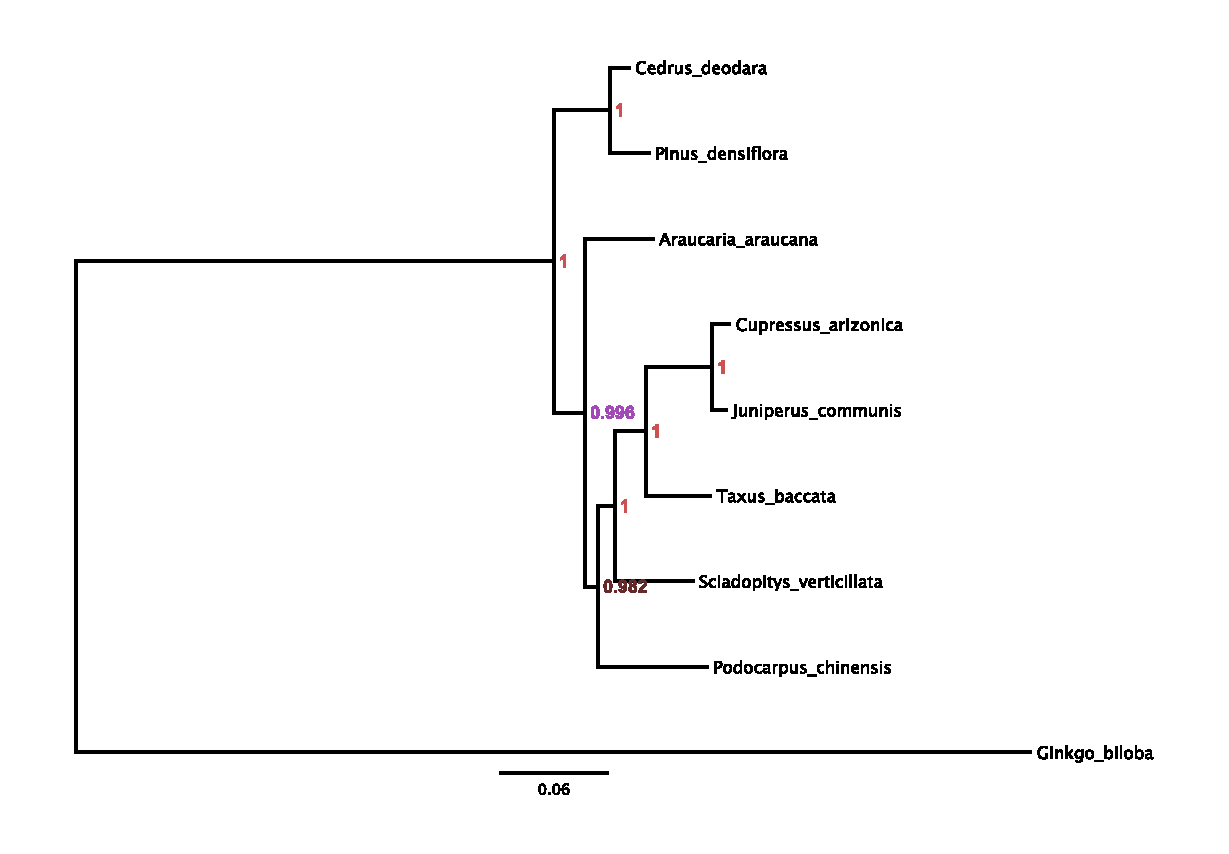
\includegraphics[width=4in,angle=0]{figures/tree_uniform_analysis.eps}}
\caption{\small The summary tree from the uniform analysis, with posterior probabilities labeled at nodes. \taha{need to make a new figure}}
\label{uniformFigTree}
\end{figure}

\bigskip
\subsection*{Exercise 1 -- Batch Mode}

If you wish to run this exercise in batch mode, the files are provided for you. 

You can carry out these batch commands by providing the file name when you execute the \cl{rb} binary in your unix terminal (this will overwrite all of your existing run files).
\exs{\cl{> rb full\_analysis.Rev}}

\bigskip
\section*{Useful Links}

\begin{itemize}
\item RevBayes: \href{https://github.com/revbayes/code}{https://github.com/revbayes/code} \\ \vspace{-7mm}
\item MrBayes: \href{http://mrbayes.sourceforge.net/}{http://mrbayes.sourceforge.net} \\ \vspace{-7mm}
\item PhyloBayes: \href{http://megasun.bch.umontreal.ca/People/lartillot/www/index.htm}{www.phylobayes.org} \\ \vspace{-7mm}
%\item BEAGLE: \href{http://code.google.com/p/beagle-lib/}{http://code.google.com/p/beagle-lib/} \\ \vspace{-7mm}
\item Tree Thinkers: \href{http://treethinkers.org/}{http://treethinkers.org} \\ \vspace{-7mm}
\end{itemize}

Questions about this tutorial can be directed to: \\\vspace{-10mm}
\begin{itemize}
\item Tracy Heath (email: \href{mailto:tracyh@berkeley.edu}{tracyh@berkeley.edu}) \\\vspace{-8mm}
\item Michael Landis (email: \href{mailto:mlandis@berkeley.edu}{mlandis@berkeley.edu}) \\\vspace{-8mm} 
\item Sebastian H\"{o}hna (email: \href{mailto:sebastian.hoehna@gmail.com}{sebastian.hoehna@gmail.com})
\end{itemize}

\href{http://creativecommons.org/licenses/by/4.0/}{
\includegraphics[scale=0.8]{figures/ccby.eps}} This tutorial was written by \href{http://phylo.bio.ku.edu/content/tracy-heath}{Tracy Heath}, \href{http://michaeljameslandis.com/}{Michael Landis}, and Sebastian H\"{o}hna; licensed under a \href{http://creativecommons.org/licenses/by/4.0/}{Creative Commons Attribution 4.0 International License}. 
(Some content in this tutorial is based on the \href{http://treethinkers.org/tutorials/phylogenetic-inference-using-mrbayes-v3-2/}{Phylogenetic Inference using MrBayes v3.2} tutorial written by Tracy Heath, Conor Meehan, and Brian Moore.)

Version dated: \today

\nocite{sukumaran10,rannala96,robert02,rodrigue08,ronquist09,Rubinstein1981,simon01,Smith1993,Suchard2005,verdinelli95,wong08,Yang2007,Yang2005,yang97b}
%\newpage

%%%%%%%%%%%%%%%%%%%%%%%%%%%%%%%%%%%%
%  REFERENCES  
%%%%%%%%%%%%%%%%%%%%%%%%%%%%%%%%%%%%

{\renewcommand{\bibsection}{\section*{Relevant References}}


\bibliography{bib_tex/master_refs}




\end{document}
